\section{Enabling Robots to Understand Incomplete Natural Language Instructions Using Commonsense Reasoning}
In~\cite{DBLP:journals/corr/TesslerGZMM16}, they introduce Language-Model-based commonsense Reasoning (LMCR), a replacement technique that permits a robot to concentrate to a linguistic communication instruction from a person's, observe the surroundings around it, and mechanically fill in info missing from the instruction mistreatment environmental context and a replacement common sensible reasoning approach. Their approach initial converts associate degree instruction provided as free linguistic communication into a type that a robot will perceive by parsing it into verb frames.

\begin{figure}[htbp]
    
    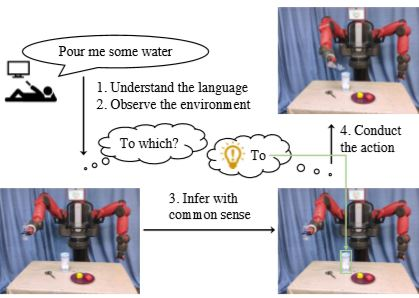
\includegraphics[width=.8\textwidth]{enable}
    \caption{A natural language controlled robot employing commonsense knowledge to interpret an instruction with missing information~\cite{DBLP:journals/corr/TesslerGZMM16} }
    \label{fig:enable}
\end{figure}
\newpage
Their approach then fills in missing data inside the instruction by observant objects in its neck of the woods and finance common wise reasoning. To be told common wise reasoning automatically, their approach distills data from huge unstructured matter corpora by coaching job a language model. Our results show the reasonableness of a automaton learning common wise data automatically from web-based matter corpora, and additionally the facility of learned common wise reasoning models in serving to a automaton to autonomously perform tasks supported incomplete communication directions.

A person provide instruction “pour him some water” however the automaton cannot perform the action while not knowing wherever to pour. When scanning the surroundings, the robot uses common sensible information to work out the missing parameters and with success perform the action.